\chapter{车道汇合群决策模型仿真}
\label{cha:sim}
% 仿真的一些综述

\section{仿真平台设计}
本课题中使用{\ttfamily Python}开发仿真程序。仿真程序大体框架如图\ref{fig:ss}。其中 {\ttfamily Vehicle}类保存车辆本身的物理状态和属性, {\ttfamily OnBoardVehicle}类保存控制车辆所需的信息和历史记录,{\ttfamily VehicleGenerator}类用于生成仿真的车辆队列并运行不同的排序方法,{\ttfamily GameLoop}类控制仿真进程,并绘制结果。
\begin{figure}
\centering
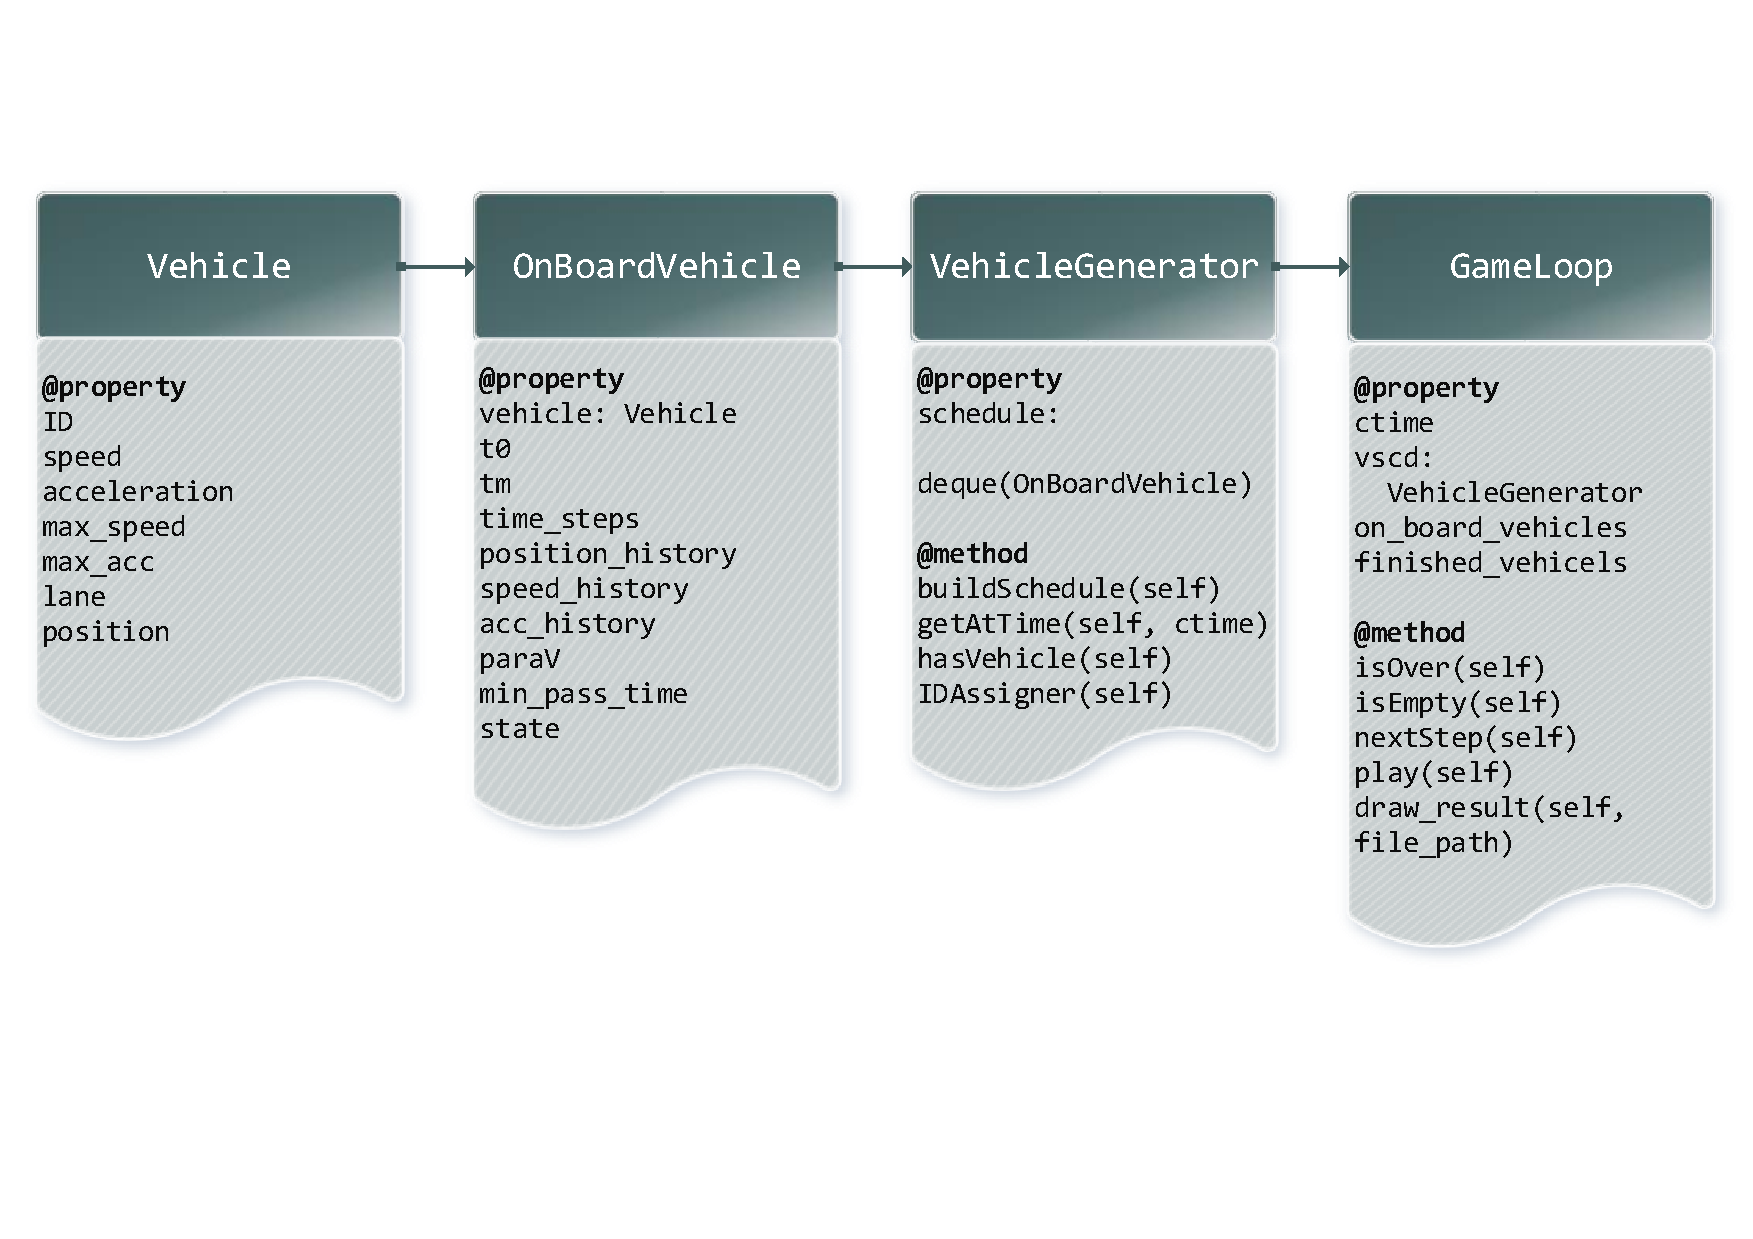
\includegraphics[width=15cm,trim={0 4cm 0 2cm},clip]{figures/software_structure.pdf}
\caption{仿真程序结构}
\label{fig:ss}
\end{figure}

为了方便进行仿真实验展示,本课题使用{\ttfamily Python}的{\ttfamily bokeh}包开发了如图\ref{fig:app}所示的仿真应用程序。
\begin{figure}
\centering
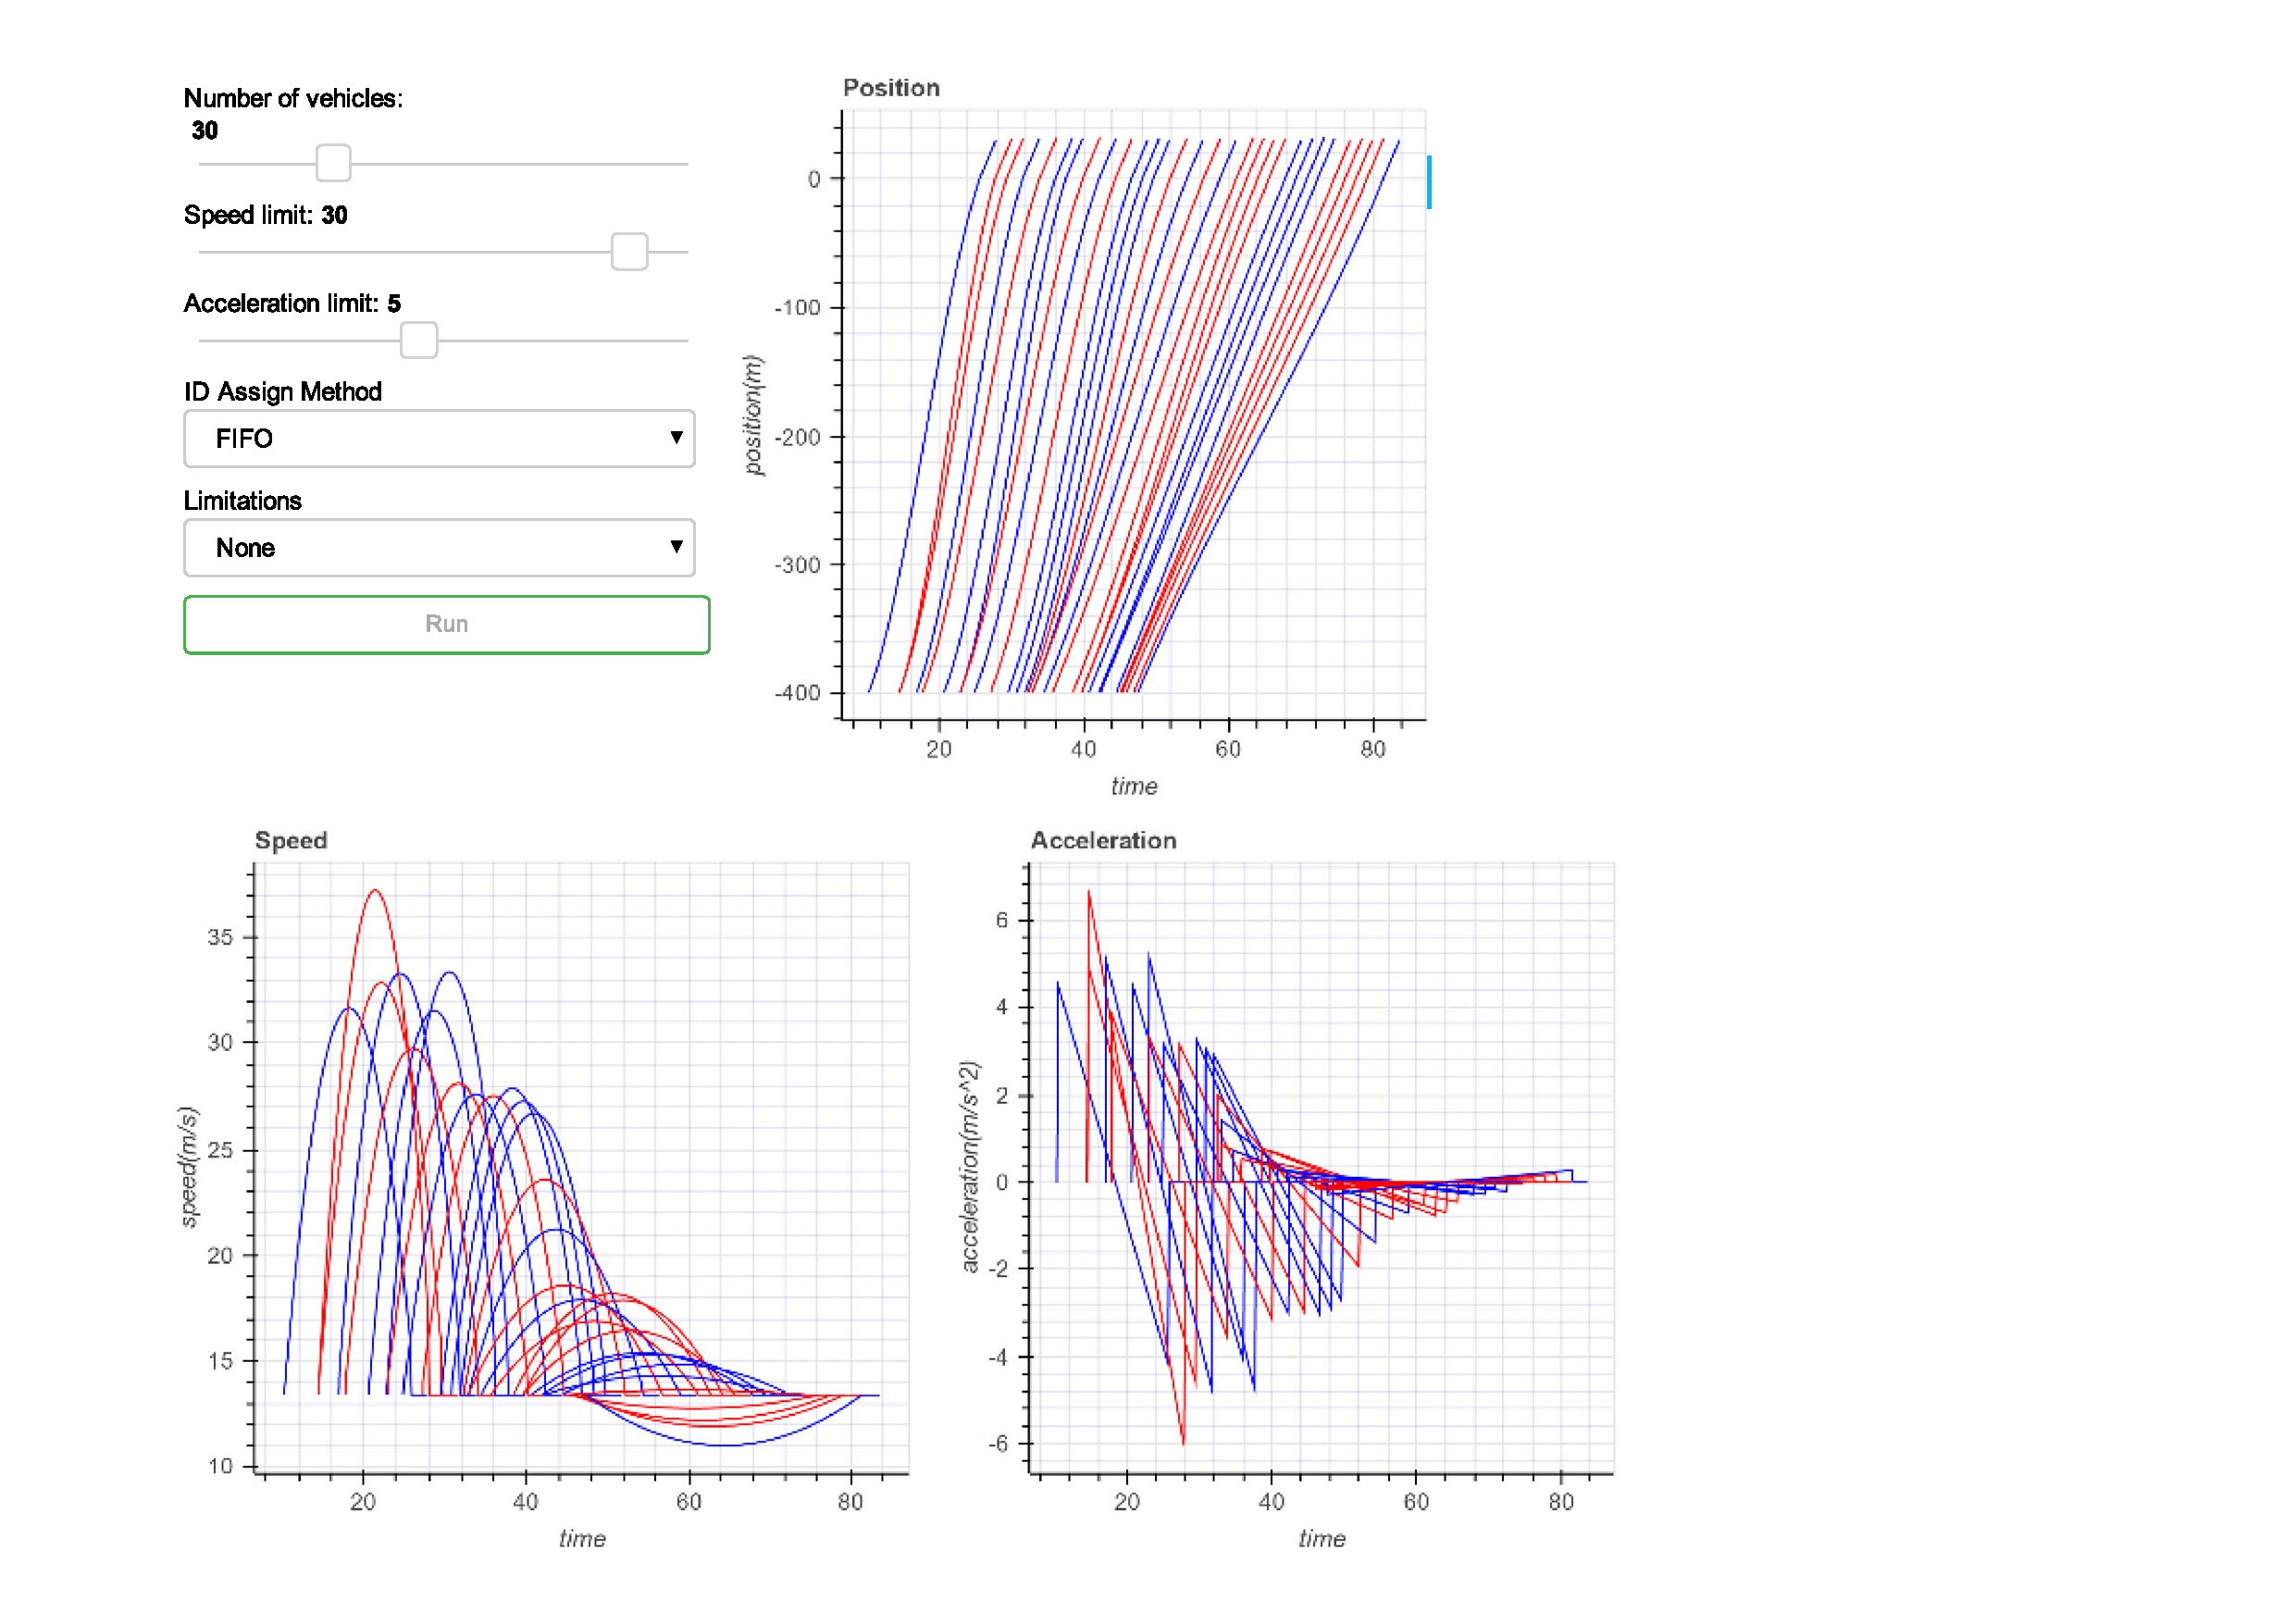
\includegraphics[angle=270,trim={0 0 0 10cm},clip,width=13cm]{figures/app.pdf}
\caption{网页APP仿真平台界面}
\label{fig:app}
\end{figure}

\section{评价指标计算}
算法效果的好坏需要数值化的评价指标来衡量。本节列举仿真程序中计算的一些评价指标及部分指标的计算方法。需要注意的是,由于后文部分仿真实验中车辆较少,而有些指标是针对宏观交通流的,例如吞吐量,这些指标列举出来是为大量数据的仿真做准备。

\textbf{平均通行时间} \ \
定义为所有车辆通过控制区及交汇区总用时的平均值,
\begin{equation}
\bar{T}(t) = \sum_{i=0}^{N(t)}(t_i^\mathrm{f}-t_i^0)/N(t),
\end{equation}
其中$N(t)$为$t$时间内通过路口的车辆总数。

\textbf{吞吐量} \ \
定义单位时间内通过路口的车辆数目为吞吐量,
\begin{equation}
Q=N(t)/t.
\end{equation}

\textbf{调和平均速度} \ \
取所有车辆自身平均速度的调和平均值为调和平均速度。
\begin{equation}
v_\mathrm{ave}(t)=N(t)/\sum_{i=0}^{N(t)}(1/\bar{v}_{i}).
\end{equation}

\textbf{平均油耗}\ \ 本文使用的油耗计算方法参照文献\inlinecite{Kamal2013Model},总油耗$\dot{f}_\mathrm{v}$由两部分构成, \ \
\begin{equation}
\dot{f}_\mathrm{v} = \dot{f}_\mathrm{cruise} + \dot{f}_\mathrm{accel},
\end{equation}
其中$\dot{f}_\mathrm{cruise}$为车辆以固定速度巡航的油耗,
\begin{equation}
\dot{f}_\mathrm{cruise}=q_0+q_1\cdot v(t)+q_2\cdot v^2(t) + q_3\cdot v^3(t).
\end{equation}
$\dot{f}_\mathrm{accel}$为加速度带来的油耗,
\begin{equation}
\dot{f}_\mathrm{accel}=u(t) \cdot (r_0 + r_1 \cdot v(t) + r_2 · v^2(t) ).
\end{equation}
按照\inlinecite{Kamal2013Model}给出的参数,系数如表\ref{tab:fuel:param}。上述公式给出的是单位时间的油耗,仿真中按照时间间隔每步计算油耗,对每辆车取平均后,再对所有车的油耗取平均即得整个系统的平均油耗,下文用$\bar{F}$表示系统的平均油耗。
\begin{table}[htbp]
\centering
\caption{油耗公式系数表}
\label{tab:fuel:param}
\begin{tabular}{ll}
\toprule[1.5pt]
$q_0$ & 0.1569 \\
$q_1$ & $2.45 \cdot 10^{−2}$ \\
$q_2$ & $−7.415 \cdot 10^{−4}$ \\
$q_3$ & $5.975 \cdot 10^{-5}$ \\
$r_0$ & $0.07224$ \\
$r_1$ & $9.681 \cdot 10^{−2}$ \\
$r_2$ & $1.075 \cdot 10^{−3}$ \\
\bottomrule[1.5pt]
\end{tabular}
\end{table}

\section{FIFO顺序仿真实验}
\textbf{相同速度进入控制区}\ \
首先检验算法是否能保证车辆进入交汇区不碰撞。不考虑速度和加速度限制,所有车辆以相同速度进入控制区,且从两车道成对进入(同一时刻两车道各有一辆车进入),一共有四辆车。在该情况下,如果不进行控制而匀速运行,两车道的车辆会发生碰撞。仿真参数设置如表\ref{tab:case1:param}。这组实验到达交汇口时间$t_i^\mathrm{m}$由式\eqref{eq:tmcase}给出,第一辆车通过时间由式\eqref{eq:tmopt}解出。
\begin{table}[htbp]
\centering
\caption{第一组仿真实验参数}
\label{tab:case1:param}
\begin{tabular}{lll}
\toprule[1.5pt]
参数符号 & 参数含义 & 参数值 \\
\midrule[1pt]
$L$ & 控制区长度 & $\SI{400.0}{m}$ \\
$S$ & 交汇区长度 & $\SI{30.0}{m}$ \\
$\delta$ & 安全距离 & $\SI{10.0}{m}$ \\
$v_0$ & 初速度 & $\SI{13.4}{m\per s}$ \\
$v_\mathrm{d}$ & 期望速度 & $\SI{25.0}{m\per s}$ \\
$t_1^0, t_2^0$ & 一、二号车进入路口时刻 & $\SI{10.0}{s}$ \\
$t_3^0, t_4^0$ & 三、四号车进入路口时刻 & $\SI{15.0}{s}$ \\
\bottomrule[1.5pt]
\end{tabular}
\end{table}

仿真结果如图\ref{fig:case1:posi}--- 图\ref{fig:case1:fuel}。其中虚线和实线分别为两条车道上的车辆。由图可见,车辆按照先进先出的顺序依次通过,并且不通车道上车辆在进入交汇区时分开的距离为$S=\SI{30}{m}$。
\begin{figure}[htbp]
\begin{minipage}{0.48\textwidth}
  \centering
  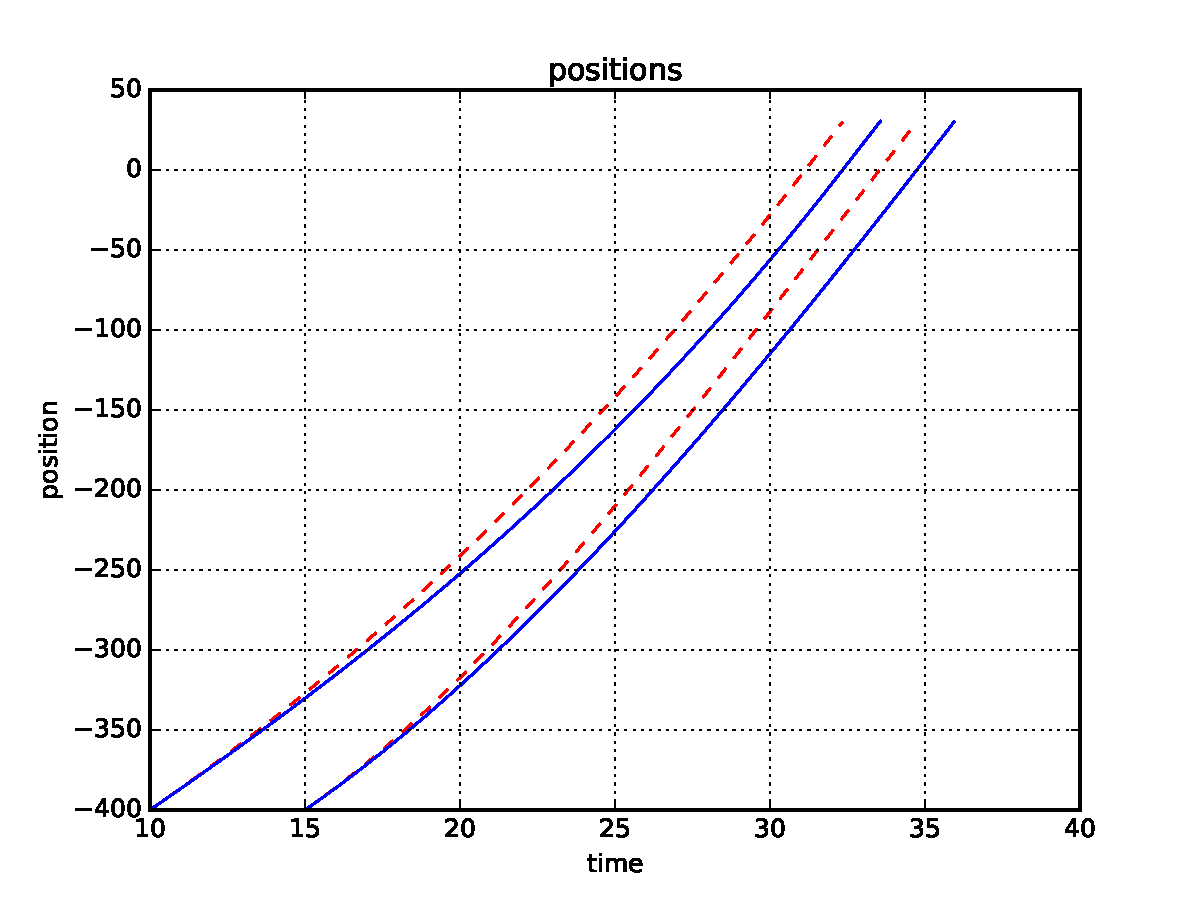
\includegraphics[height=6cm]{figures/sim_case1/posi.pdf}
  \caption{位移-时间关系图}
  \caption*{\small (第一组)}
  \label{fig:case1:posi}
\end{minipage}\hfill
\begin{minipage}{0.48\textwidth}
  \centering
  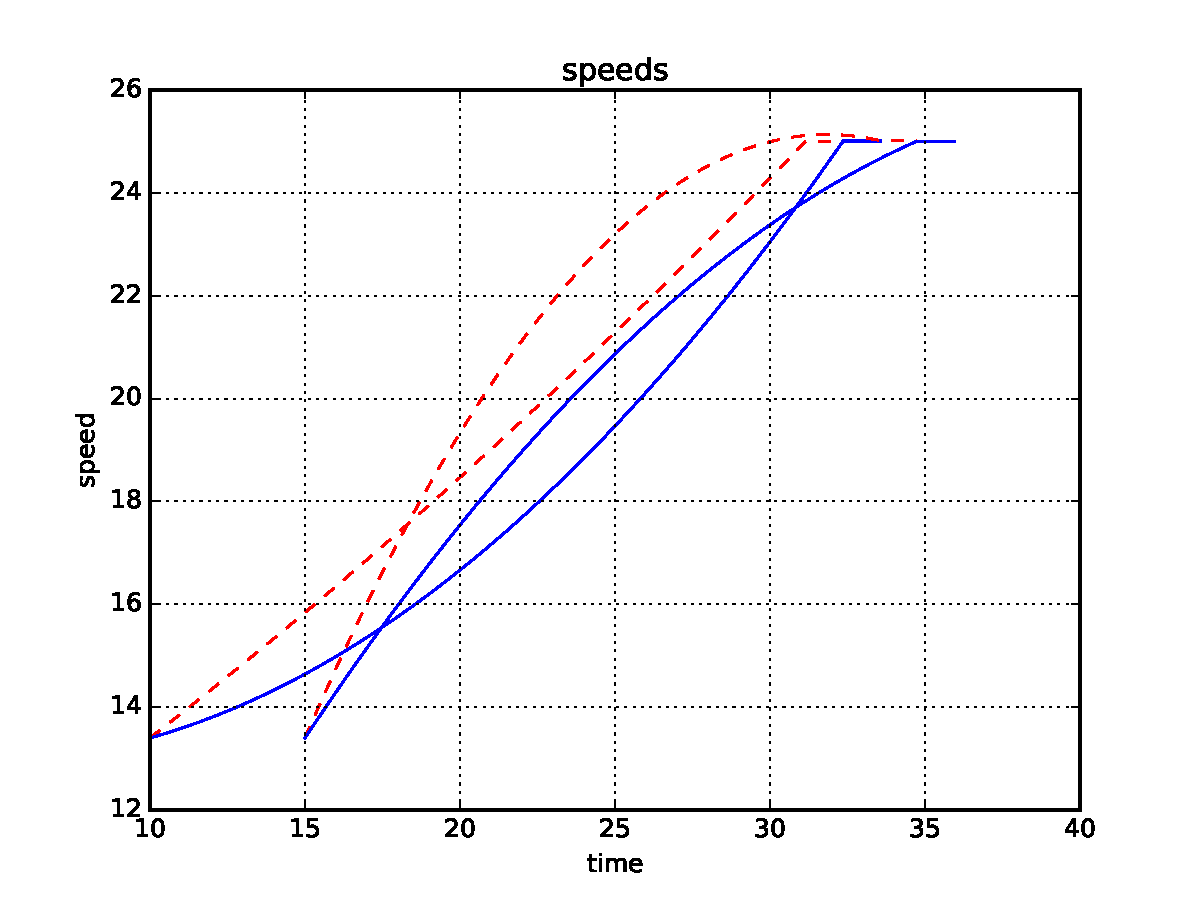
\includegraphics[height=6cm]{figures/sim_case1/speed.pdf}
  \caption{速度-时间关系图}
  \caption*{\small (第一组)}
  \label{fig:case1:speed}
\end{minipage}
\end{figure}
\begin{figure}[htbp]
\begin{minipage}{0.48\textwidth}
  \centering
  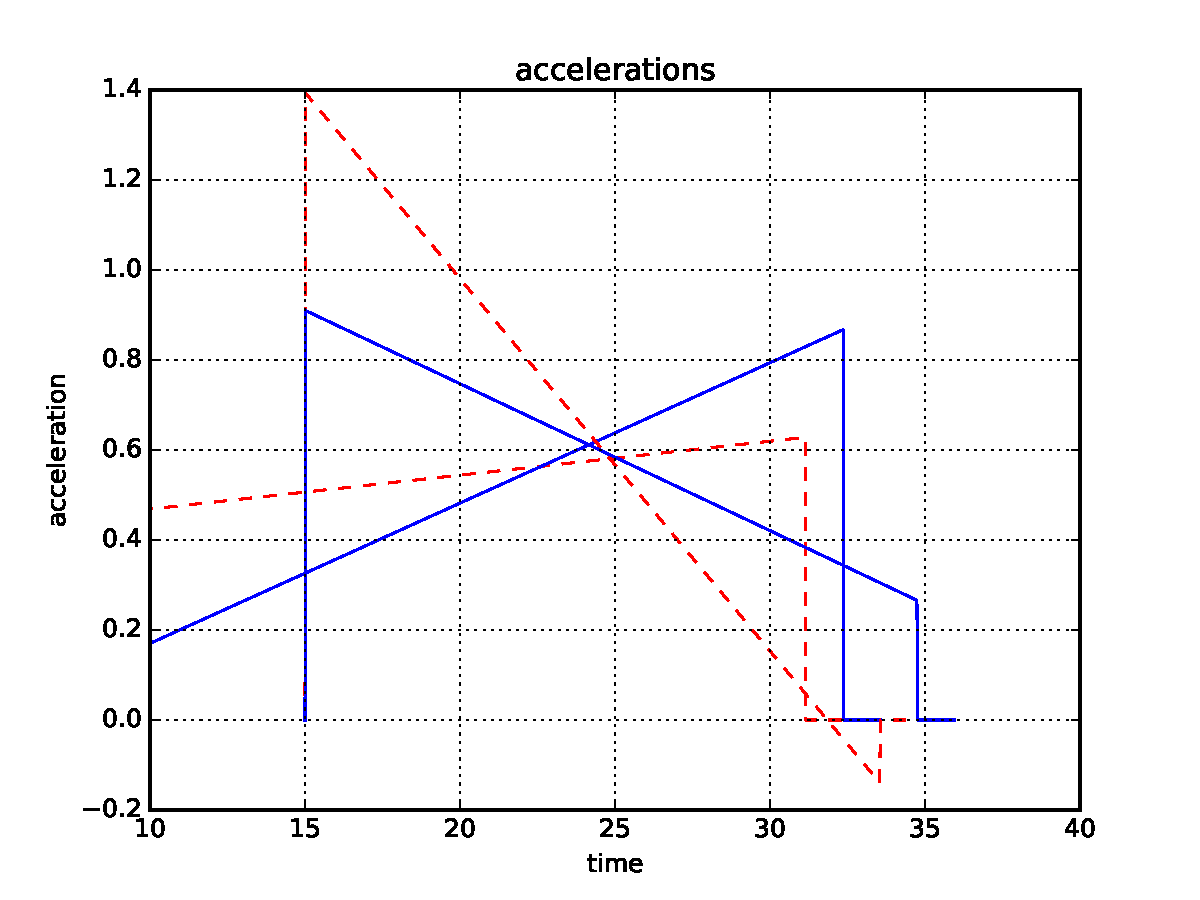
\includegraphics[height=6cm]{figures/sim_case1/acc.pdf}
  \caption{加速度-时间关系图}
  \caption*{\small (第一组)}
  \label{fig:case1:acc}
\end{minipage}\hfill
\begin{minipage}{0.48\textwidth}
  \centering
  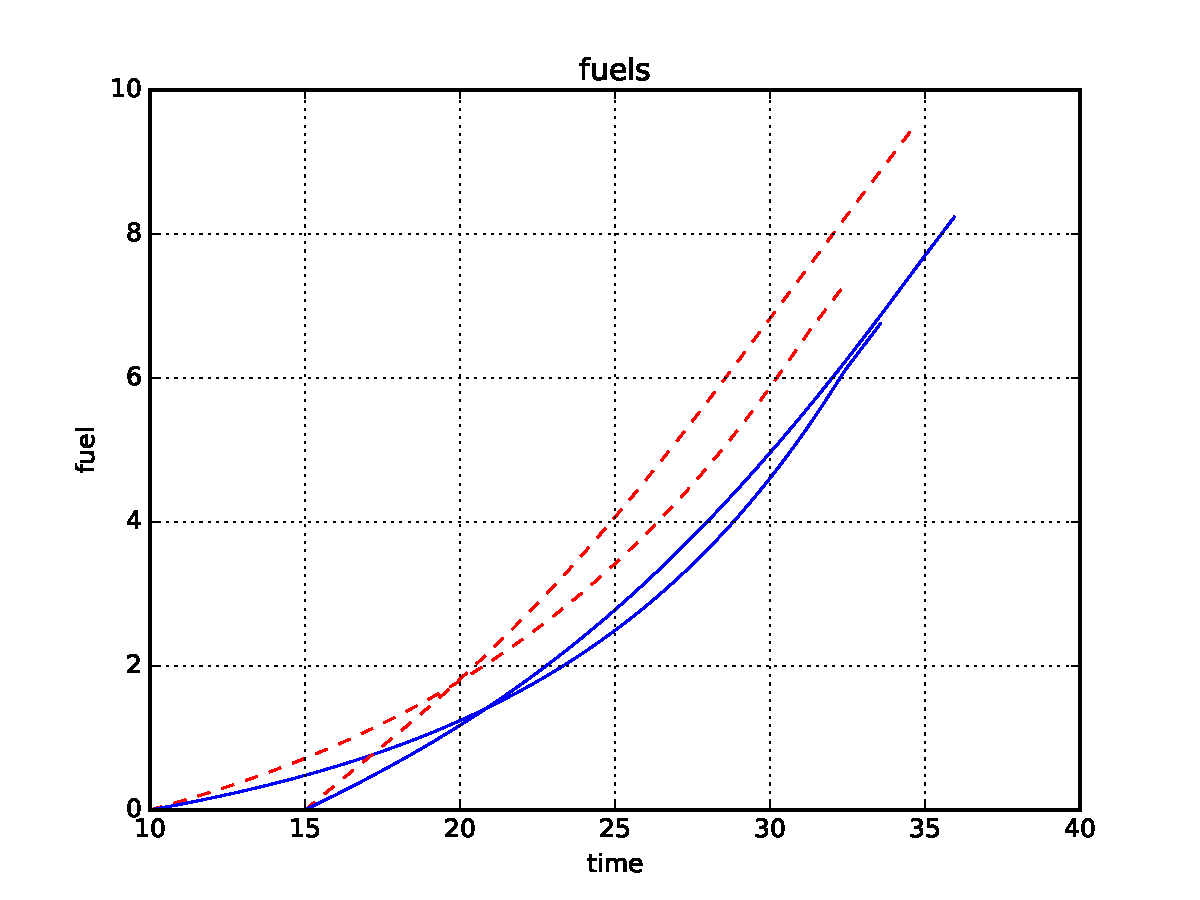
\includegraphics[height=6cm]{figures/sim_case1/fuel.pdf}
  \caption{油耗-时间关系图}
  \caption*{\small (第一组)}
  \label{fig:case1:fuel}
\end{minipage}
\end{figure}

\textbf{主辅路不同速度进入控制区}
\label{ssec:diffv}
\ \ 其次研究主路与辅路按照不同初速度(同车道进入车辆初速度仍然相同)进入控制区时的情况,其中各个车道车辆按照固定的时间差进入控制区。仿真参数设置如表\ref{tab:case2:param}。仿真结果如图\ref{fig:case2:posi}--- 图\ref{fig:case2:fuel}。其中虚线表示主路上车辆,实线表示辅路上车辆。由图可以观察到以下现象:
\begin{enumerate}[label=(\arabic*), wide=\parindent]
% \begin{enumerate}
\item 同车道车辆在通过交汇区时保持了安全距离,比不同车道的车辆距离小;
\item 主车道的车辆需要减速等待先进入控制区的辅路车通过路口。
\end{enumerate}
\begin{table}[htbp]
\centering
\caption{第二组仿真实验参数}
\label{tab:case2:param}
\begin{tabular}{lll}
\toprule[1.5pt]
参数符号 & 参数含义 & 参数值 \\
\midrule[1pt]
$L$ & 控制区长度 & $\SI{400.0}{m}$ \\
$S$ & 交汇区长度 & $\SI{30.0}{m}$ \\
$\delta$ & 安全距离 & $\SI{10.0}{m}$ \\
$v_0^\mathrm{m}$ & 主路初速度 & $\SI{25.0}{m\per s}$ \\
$v_0^\mathrm{a}$ & 主路初速度 & $\SI{15.0}{m\per s}$ \\
$v_\mathrm{d}$ & 期望速度 & $\SI{25.0}{m\per s}$ \\
\bottomrule[1.5pt]
\end{tabular}
\end{table}

\begin{figure}[htbp]
\begin{minipage}{0.48\textwidth}
  \centering
  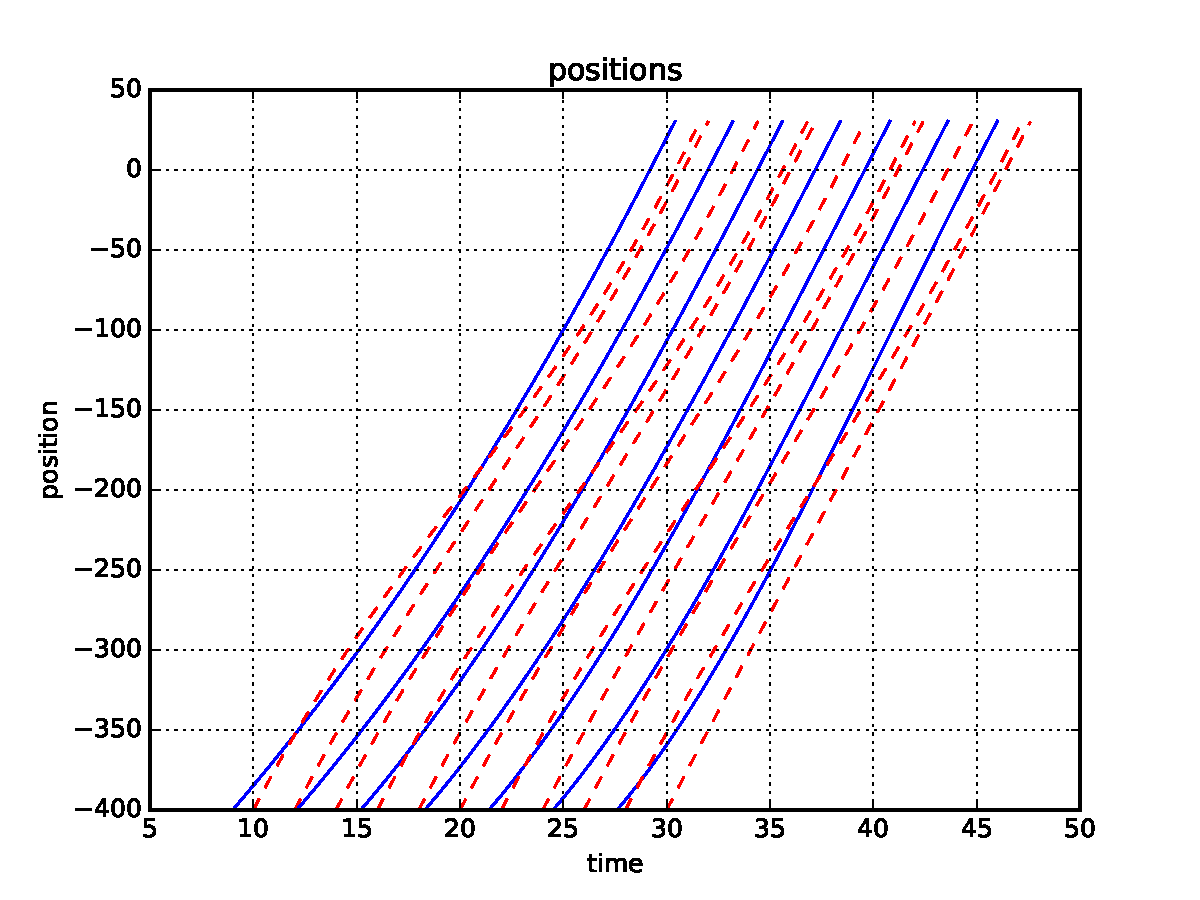
\includegraphics[height=5.4cm]{figures/sim_case2/posi.pdf}
  \caption{位移-时间关系图}
  \caption*{\small (第二组)}
  \label{fig:case2:posi}
\end{minipage}\hfill
\begin{minipage}{0.48\textwidth}
  \centering
  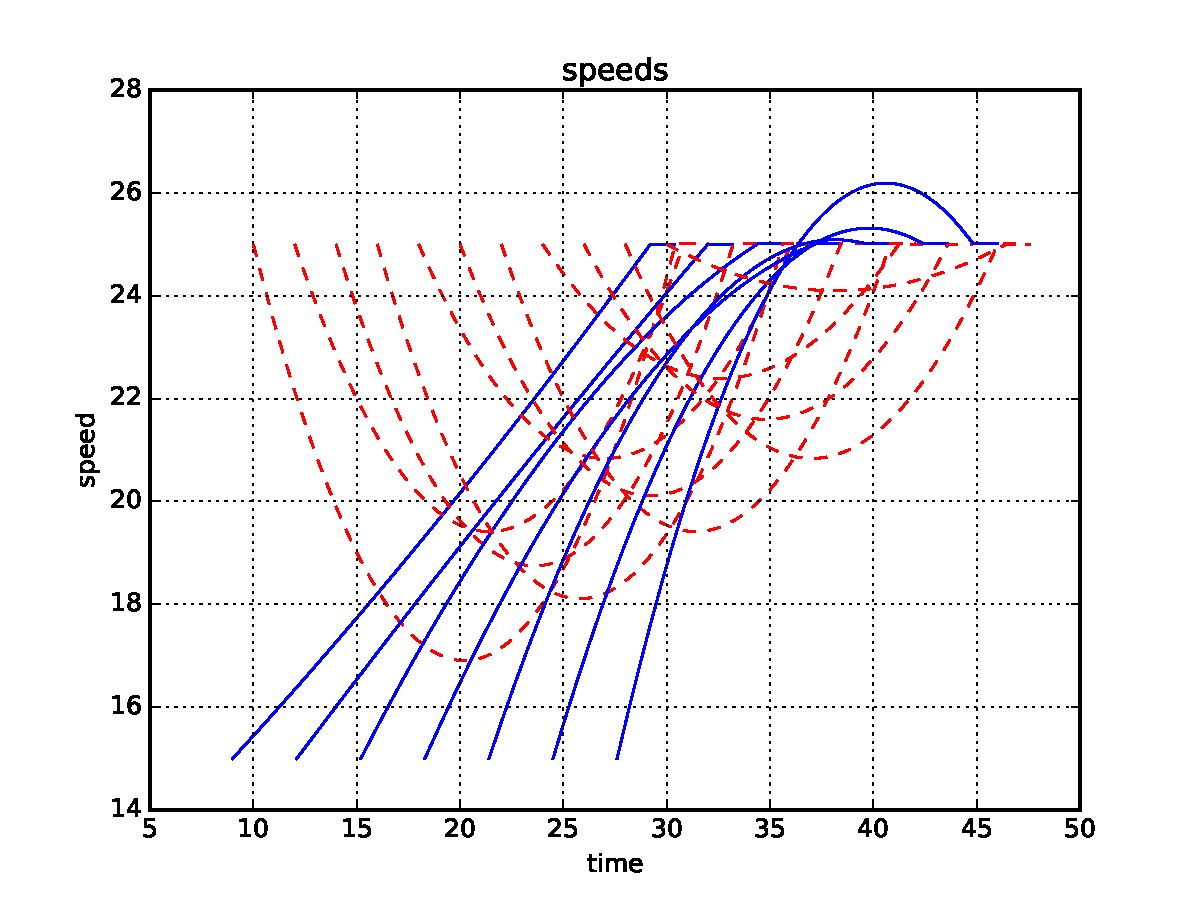
\includegraphics[height=5.4cm]{figures/sim_case2/speed.pdf}
  \caption{速度-时间关系图}
  \caption*{\small (第二组)}
  \label{fig:case2:speed}
\end{minipage}
\end{figure}
\begin{figure}[htbp]
\begin{minipage}{0.48\textwidth}
  \centering
  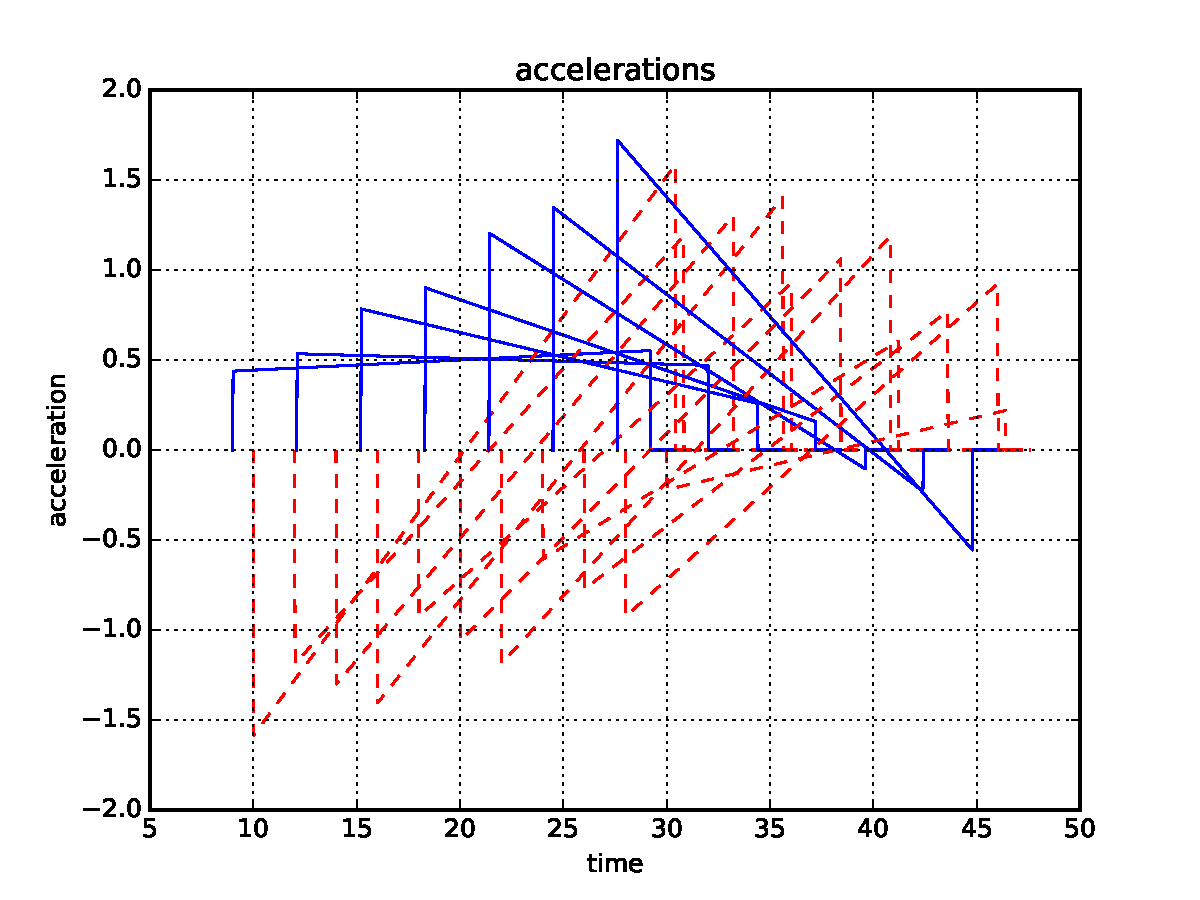
\includegraphics[height=5.4cm]{figures/sim_case2/acc.pdf}
  \caption{加速度-时间关系图}
  \caption*{\small (第二组)}
  \label{fig:case2:acc}
\end{minipage}\hfill
\begin{minipage}{0.48\textwidth}
  \centering
  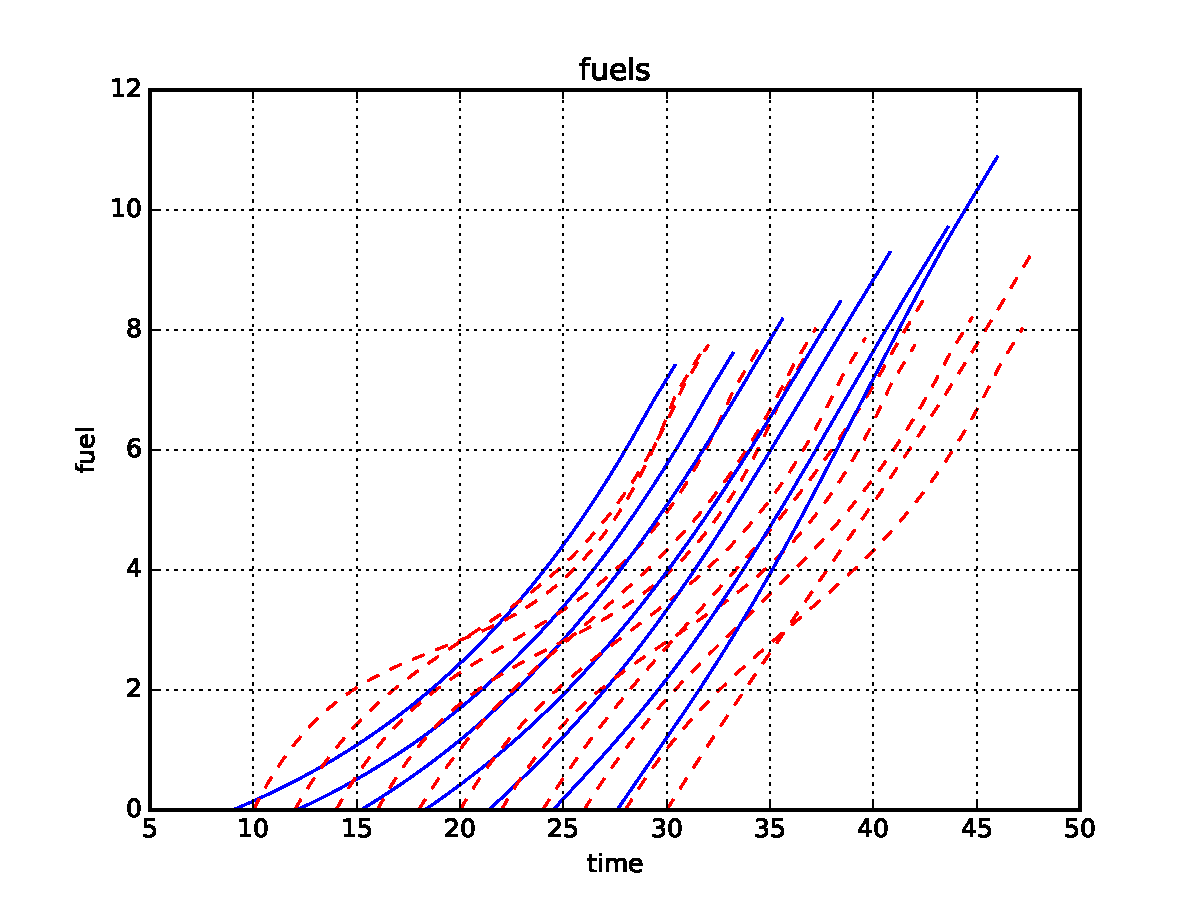
\includegraphics[height=5.4cm]{figures/sim_case2/fuel.pdf}
  \caption{油耗-时间关系图}
  \caption*{\small (第二组)}
  \label{fig:case2:fuel}
\end{minipage}
\end{figure}

% \subsection{随机速度进入控制区}

\section{OTM顺序仿真实验}
\textbf{硬变化实验}\ \
\ref{ssec:diffv}节中,对于主路速度高于辅路的情况,主路车辆需要等待辅路通行方能通过。本节中对文章里提出的最优通行时间(OTM)顺序进行仿真,参数同表\ref{tab:case2:param},仿真结果如图\ref{fig:case3:posi}--- 图\ref{fig:case3:fuel},其中虚线表示主路上车辆,实线表示辅路上车辆。由图可以观察到,在主路上后进入的车辆能够先于辅路上车辆通过路口,辅路车辆由于通行时间$t_\mathrm{m}$被迫延长,需要重新计算控制量来适应新的$t_\mathrm{m}$。但由图可以看出一个明显的问题,辅路车辆在每次主路有车辆进入时,都有可能被向后排斥,导致控制量多次改变。这与理想状态的最优控制显然有差距。将这种变化控制量的方式称作\textbf{硬变化}。

\begin{figure}[htbp]
\begin{minipage}{0.48\textwidth}
  \centering
  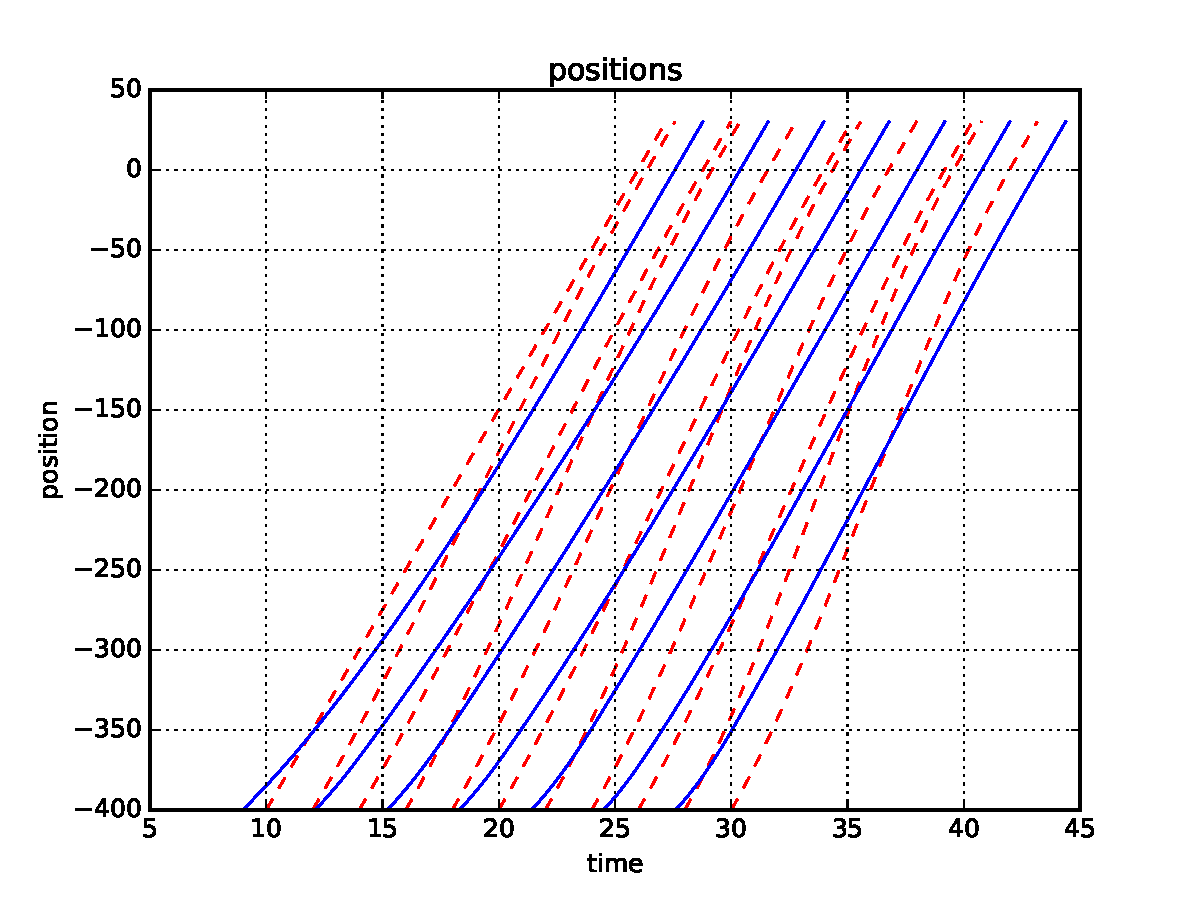
\includegraphics[height=5.4cm]{figures/sim_case3/posi.pdf}
  \caption{位移-时间关系图}
  \caption*{\small (硬变化)}
  \label{fig:case3:posi}
\end{minipage}\hfill
\begin{minipage}{0.48\textwidth}
  \centering
  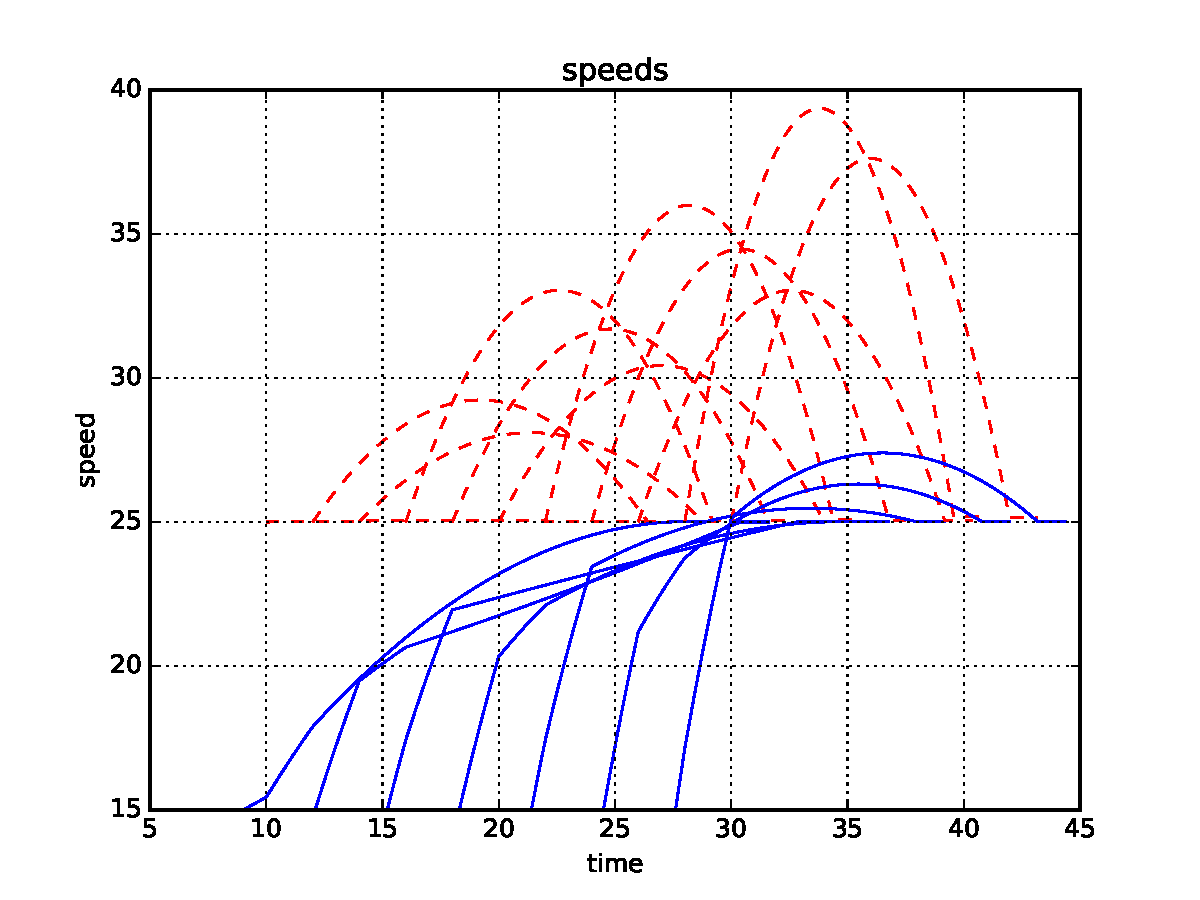
\includegraphics[height=5.4cm]{figures/sim_case3/speed.pdf}
  \caption{速度-时间关系图}
  \caption*{\small (硬变化)}
  \label{fig:case3:speed}
\end{minipage}
\end{figure}
\begin{figure}[htbp]
\begin{minipage}{0.48\textwidth}
  \centering
  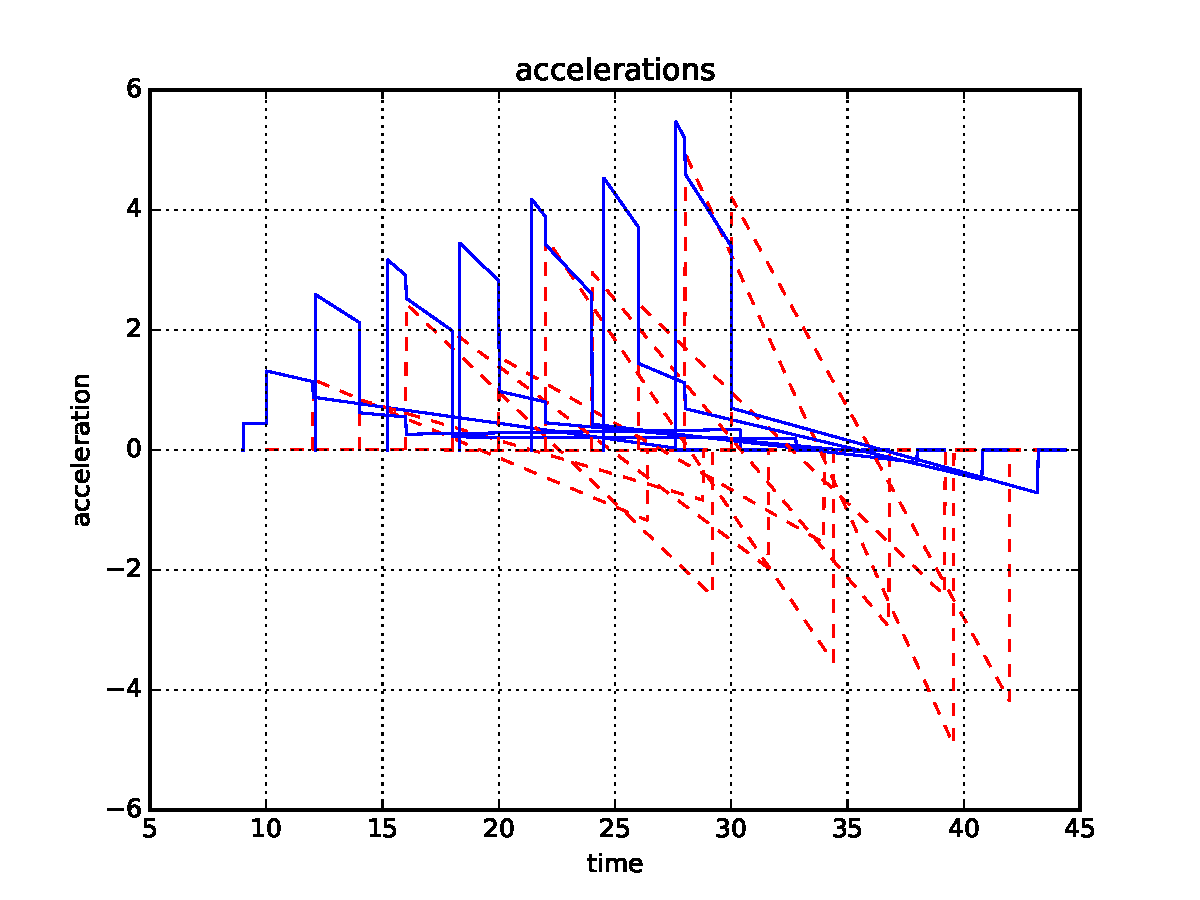
\includegraphics[height=5.4cm]{figures/sim_case3/acc.pdf}
  \caption{加速度-时间关系图}
  \caption*{\small (硬变化)}
  \label{fig:case3:acc}
\end{minipage}\hfill
\begin{minipage}{0.48\textwidth}
  \centering
  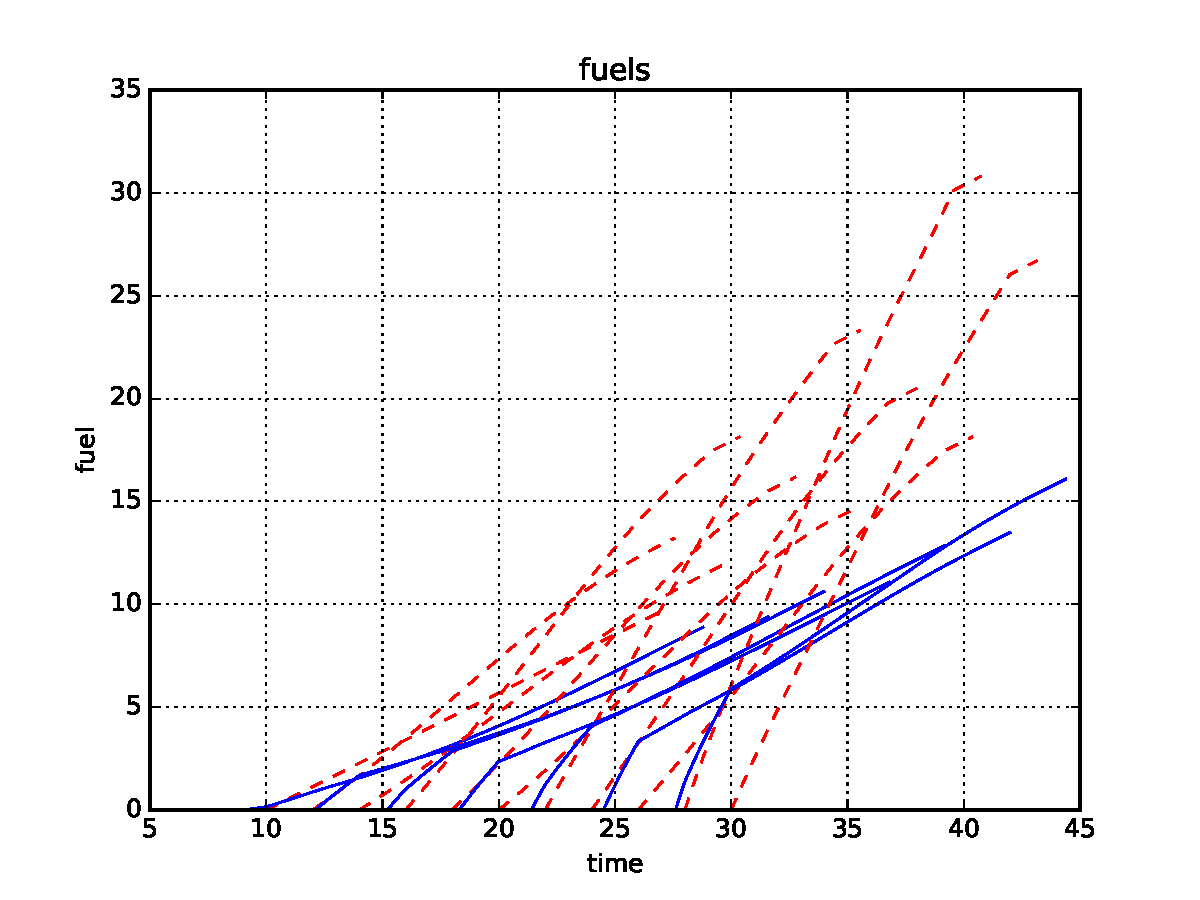
\includegraphics[height=5.4cm]{figures/sim_case3/fuel.pdf}
  \caption{油耗-时间关系图}
  \caption*{\small (硬变化)}
  \label{fig:case3:fuel}
\end{minipage}
\end{figure}

\textbf{软变化实验}\ \
为了减小控制量硬变化造成的能量损耗,辅路上车辆应该提前考虑到主路上车辆可能出现并将其向后排斥的情况,因此应在式\ref{eq:tmcase}给出的通行时间基础上适当延长。这里提出一种将辅路$t_\mathrm{m}$延长至终端自由状态下最优$t_\mathrm{m}$的方案,称这种控制量变化方式为\textbf{软变化}。仿真参数同表\ref{tab:case2:param},仿真结果如图\ref{fig:case4:posi}--- 图\ref{fig:case4:fuel},其中虚线表示主路上车辆,实线表示辅路上车辆。由图可见,辅路车辆按照最优$t_\mathrm{m}$通过路口,且没有受到主路车辆的影响。在随机生成车辆的实验中发现,在个别情况下辅路车辆还是会调整控制量,但是调整的概率很小。

\begin{figure}[htbp]
\begin{minipage}{0.48\textwidth}
  \centering
  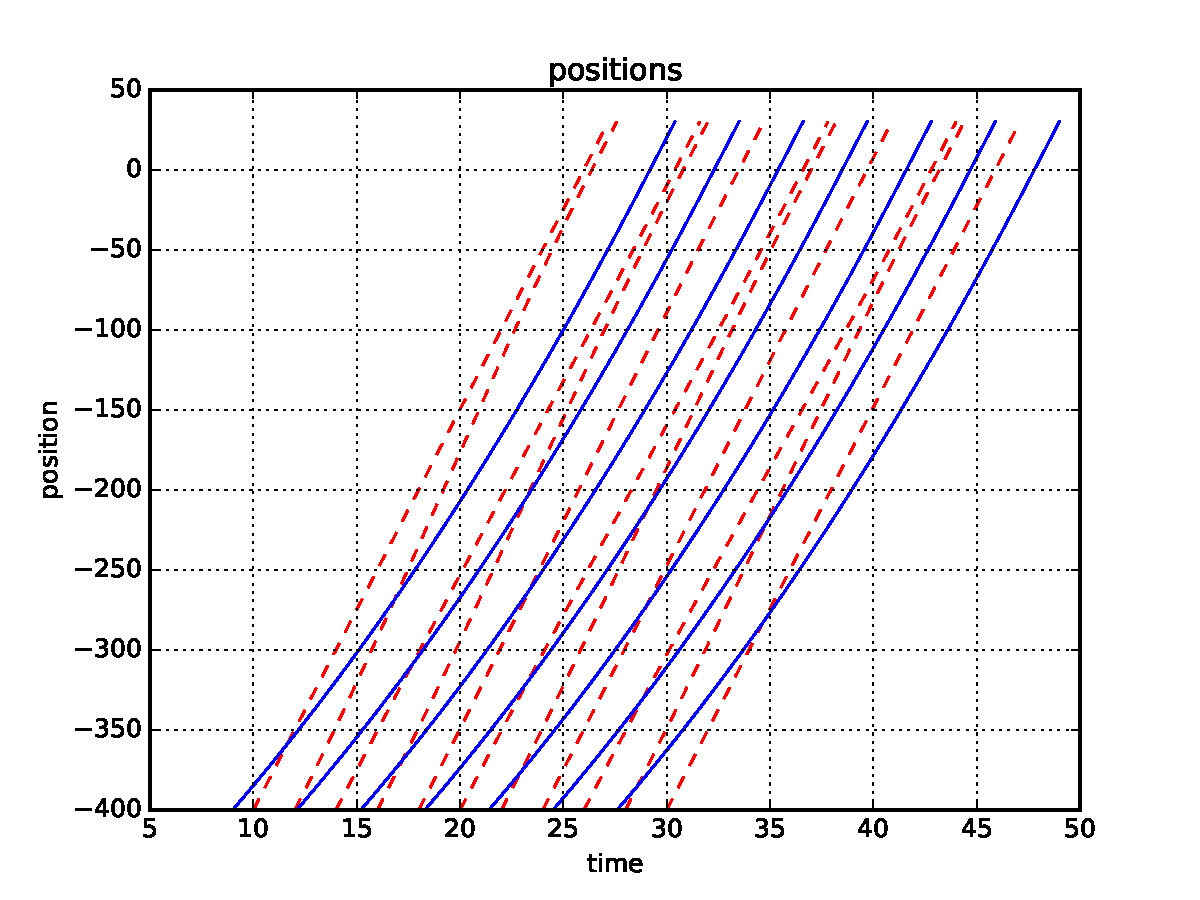
\includegraphics[height=5.4cm]{figures/sim_case4/posi.pdf}
  \caption{位移-时间关系图}
  \caption*{\small (软变化)}
  \label{fig:case4:posi}
\end{minipage}\hfill
\begin{minipage}{0.48\textwidth}
  \centering
  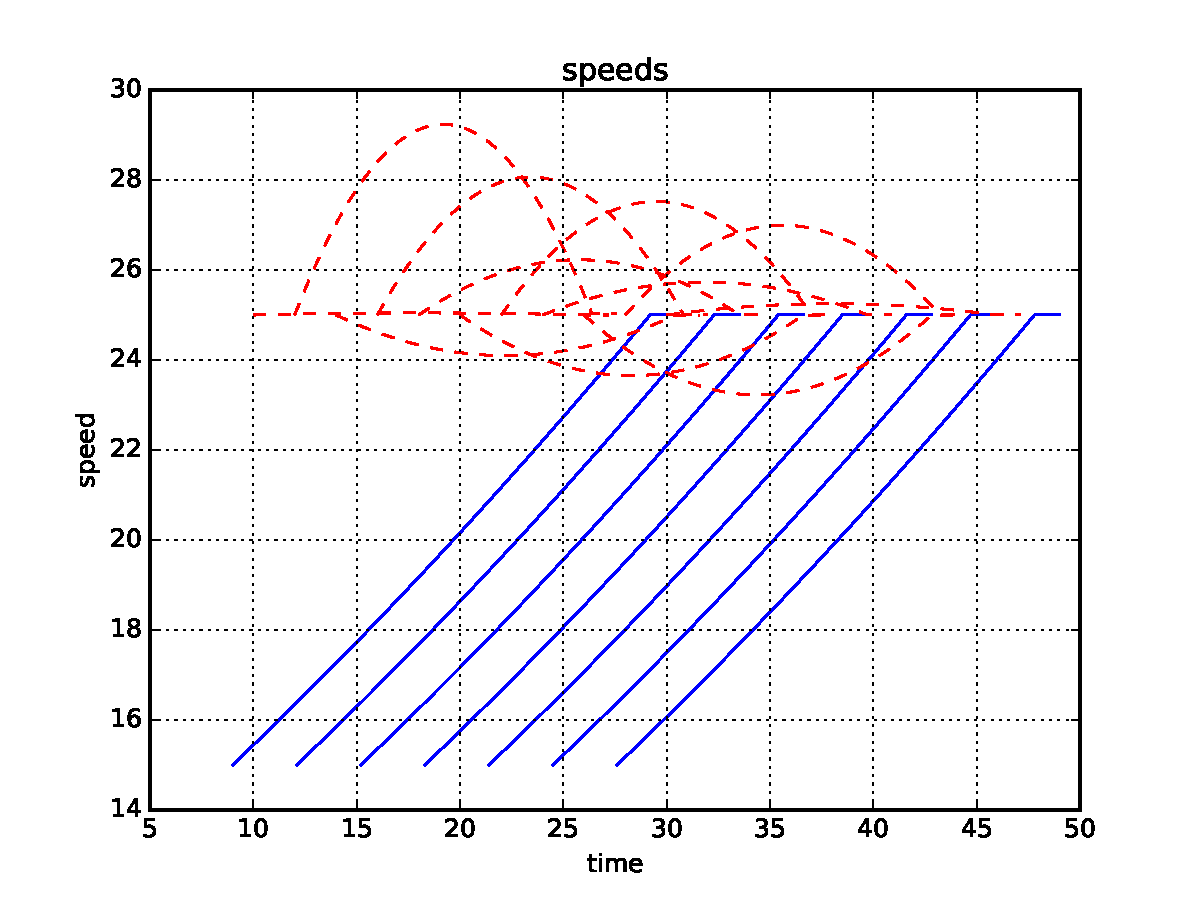
\includegraphics[height=5.4cm]{figures/sim_case4/speed.pdf}
  \caption{速度-时间关系图}
  \caption*{\small (软变化)}
  \label{fig:case4:speed}
\end{minipage}
\end{figure}
\begin{figure}[htbp]
\begin{minipage}{0.48\textwidth}
  \centering
  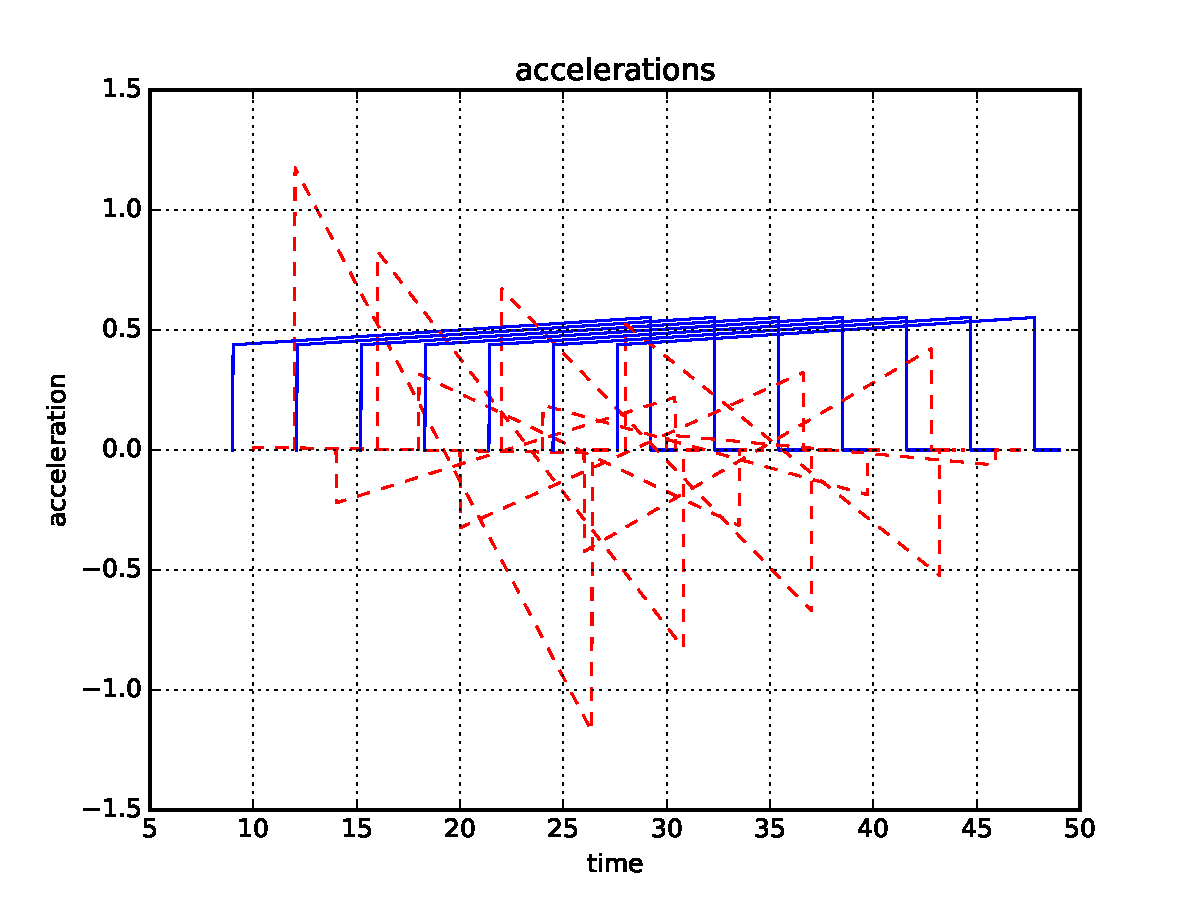
\includegraphics[height=5.4cm]{figures/sim_case4/acc.pdf}
  \caption{加速度-时间关系图}
  \caption*{\small (软变化)}
  \label{fig:case4:acc}
\end{minipage}\hfill
\begin{minipage}{0.48\textwidth}
  \centering
  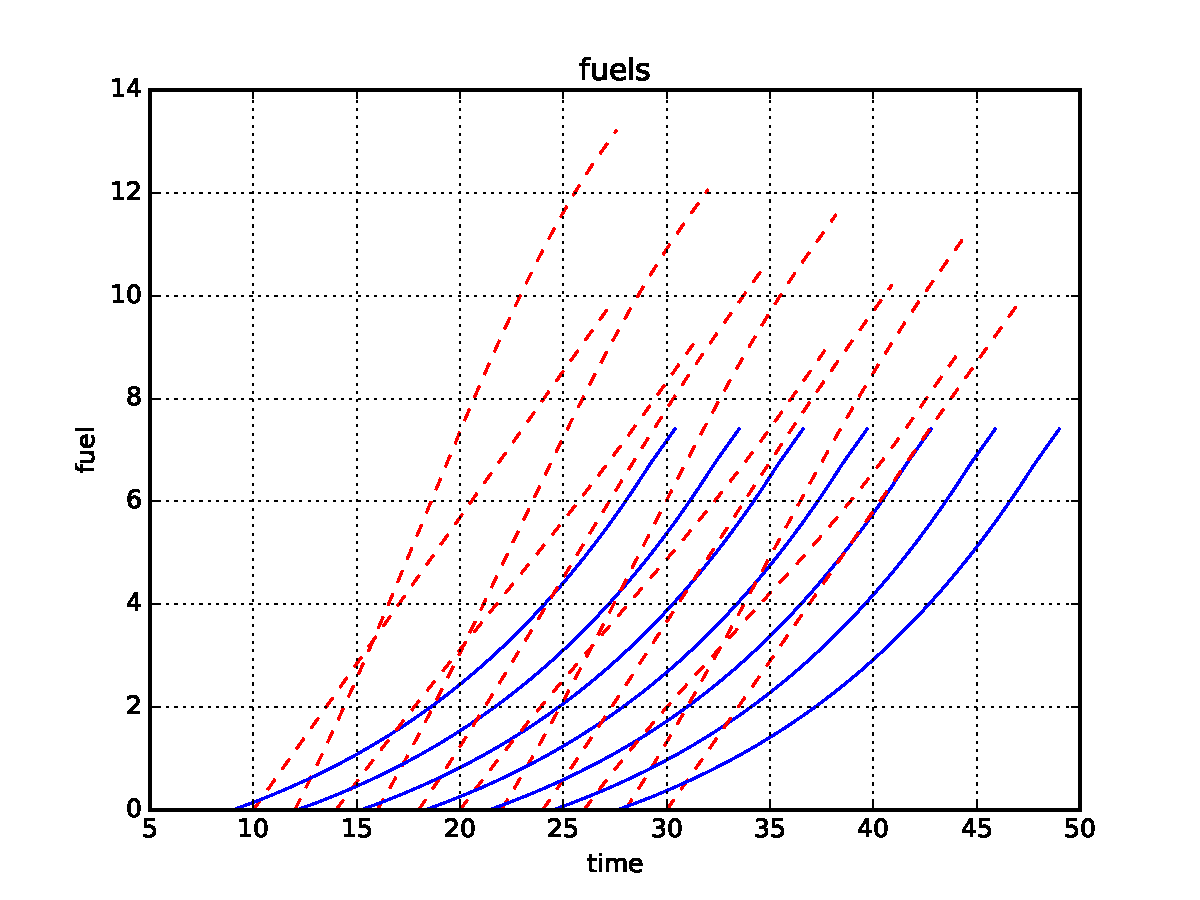
\includegraphics[height=5.4cm]{figures/sim_case4/fuel.pdf}
  \caption{油耗-时间关系图}
  \caption*{\small (软变化)}
  \label{fig:case4:fuel}
\end{minipage}
\end{figure}

将先进先出的排序方法相比,评价指标的变化表如表\ref{tab:compare}。由表可见,FIFO算法的运行效率最低,但油耗比较节省,硬变化的OTM顺序算法运行效率最高,但非常费油。软变化的FIFO算法介于二者中间,能够达到比FIFO稍高的通行效率,同时油耗与FIFO算法接近。
\begin{table}[htbp]
\centering
\caption[仿真实验结果比较表]{仿真实验结果比较表。其中$\bar{T}$,$Q$,$v_\mathrm{ave}$,$\bar{F}$分别为平均通行时间,吞吐量,调和平均速度和平均油耗。OTM(Hard)为硬变化的OTM顺序算法,OTM(Soft)为软变化的OTM顺序算法。}
\label{tab:compare}
\begin{tabular}{llll}
\toprule[1.5pt]
\diagbox[width=10em]{评价指标}{仿真算法} & FIFO & OTM(Hard) & OTM(Soft) \\
\midrule[1pt]
$\quad \bar{T}$($\si{s}$)  & 19.76 & 16.08 & 18.63 \\
$\quad Q$($\si{ve\per s}$)  & 0.4663 & 0.5236 & 0.4616 \\
$\quad v_\mathrm{ave}$($\si{km\per h}$)  & 78.403 & 96.265 & 83.139 \\
$\quad \bar{F}$($\si{ml\per ve}$) & 8.3242 & 15.8812 & 9.2989 \\
\bottomrule[1.5pt]
\end{tabular}
\end{table}

% \section{改进的优先到达序列仿真}
% \subsection{排序原理}
% \subsection{时间目标优先}
% \subsection{系统能量目标优先}

% \chapter{群决策模型改进}
% (有时候由于信息不准或延迟,可能控制区会撞)
% \section{碰撞紧急修正处理}
% \subsection{修正必要性与原理}
% \subsection{带有修正的系统仿真}
% \section{}